\section{Zweipuls-Gleichrichter}

\subsection{B2U: Ungesteuerter Zweipuls-Gleichrichter}

% --- bestehende Grafik: Brückenschaltung ---
\begin{figure}[h]
\centering
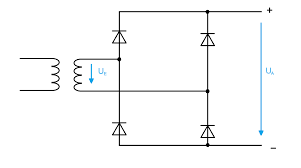
\includegraphics[width=0.6\linewidth]{images/B2U.png}
\caption{Zweipuls-Brückengleichrichter B2U}
\end{figure}

Der B2U-Gleichrichter ist eine vollwellige Brückenschaltung mit vier Dioden.
Die Pulszahl beträgt $p=2$.

Momentane Ausgangsspannung:
\[
u_d(t) = |u_s(t)|
\]

Mittelwert:
\[
\cbl{\overline{u_d} = \frac{2\hat U}{\pi}}
\]

Effektivwert:
\[
\cbl{U_{d,\mathrm{RMS}} = \frac{\hat U}{\sqrt{2}}}
\]

Eigenschaften:
\begin{itemize}
    \item Keine Stellmöglichkeit
    \item Geringere Welligkeit als M1U
    \item Standard-Gleichrichtertopologie
\end{itemize}

% --- bestehende Grafik: Spannungsverlauf ---
\begin{center}
    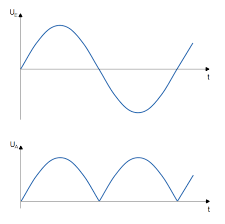
\includegraphics[width=0.85\linewidth]{images/B2U_verlauf.png}
\end{center}